% Sample LaTeX file for creating a paper in the Morgan Kaufmannn two
% column, 8 1/2 by 11 inch proceedings format.


\documentclass[]{article}
\usepackage{proceed2e}
\usepackage{cite}
\usepackage{xr}
\externaldocument[A-]{Appendix_GMCM_UAI}


% Set the typeface to Times Roman
\usepackage{times}
\usepackage{float} % for figure placement
\usepackage{amsmath}
\usepackage{graphicx}

\title{An Expectation Maximization Algorithm for Gaussian Mixture Copula Models}

%\author{ {\bf Ashuosh Tewari} \\
%ExxonMobil Research and Engineering Company\\
%Annandale, NJ, USA \\
%\And
%{\bf Anders Ellern Bilgrau} \\
%Department of Mathematical Sciences\\
%Aalborg University, Denmark
%}


\begin{document}

\DeclareRobustCommand{\native_llDenom}[1] {\prod\limits_{r=1}^{d}\psi_{r}\left(\Psi^{-1}_{r} \left( u_r{#1} \right);\beta_r \right) }

\DeclareRobustCommand{\llDenom}[1] {\prod\limits_{r=1}^{d}\psi_{r}\left(z_r({#1});\beta_r \right) }
%\DeclareRobustCommand{\invCDF}[1]{ \Psi_{\circ}^{-1}\left(\textbf{u}({#1}) \right) } 
\DeclareRobustCommand{\invCDF}[1]{ \textbf{z}({#1}) }

\DeclareRobustCommand{\erf}{\textmd{erf}}
\DeclareRobustCommand{\AltllDenom}[1] {\log \left( \psi_{r}\left(\Psi^{-1}_{r} \left( u_r{#1} \right);\beta_r \right) \right) }

\DeclareRobustCommand{\zbar}[1] {\bar{\textbf{z}}({#1})}

\DeclareRobustCommand{\ma_zbar}[2] {\bar{\textbf{z}}_{#1}(#2)}

\DeclareRobustCommand{\der}[2] {\frac{d \left({#2}\right)}{d{#1}}}


\maketitle

\begin{abstract}
We present an expectation-maximization (EM) algorithm for a promising new class of models called Gaussian mixture copula models (GMCMs). GMCMs provide an attractive alternative to widely used Gaussian Mixture Models (GMMs) as a generative distribution for continuous random variables that exhibit multi-modal and non-normal behaviour. Like other copula-based model, the strength of GMCMs comes from the ability to separate the learning of marginal models of the random variables from that of the dependence between them.  Despite this flexibility and its potential impact on modeling real-world data, learning GMCM parameters is hard. A complicated likelihood function and the over-reliance of gradient-based maximum likelihood methods on numerical approximations, can make the model cost prohibitive and possibly vulnerable to numerical errors. We derive an EM algorithm which, in addition to reducing the runtime complexity, is devoid of any approximation. We supplement our analysis with some practical examples and make a case for GMCM's wide-spread applicability.	
\end{abstract}

\section{Introduction}\label{sec:Intro}
Modeling multivariate data is a fundamental problem of interest in many domains. From a probabilistic viewpoint, it amounts to defining a generative process that best explains the observed data. Hence, there is a constant search for novel and  meaningful probabilistic generative models that can adequately explain multitude of real-world datasets, while imposing minimal assumptions. Copula functions provide a unique framework to model multivariate data that allows complete control on the marginal behaviour of the random variables; while capturing the interactions between them separately. This decoupling can be significant from the perspective of numerous practical applications. For instance, data generated by a physical process, may have strict constraints over the marginal distributions of certain variables stemming from the underlying, perhaps, unknown physics. Ideally, any effort to model such data should adhere to these constraints. However, in the pursuit of finding a joint model of the variables, one may end up with inconsistent marginal models. There is a recent surge in the research to find the synergy between copula theory and machine learning to overcome such challenges. Elidan ~\cite{Elidan2013} provides an excellent review of the state of the art in use of copulas in machine learning approaches.

In this paper, we focus on a specific class of multivariate problems where 1) all the random variables are continuous and 2) the joint distribution exhibits a multi-modal behaviour. Gaussian mixture models (GMMs) have been prolifically used for  modeling such data sets, thanks to their simplicity and an efficient algorithm to learn the parameters. However, the assumption of jointly normally distributed components is frequently violated, which may have significant practical ramifications. Gaussian mixture copula models (GMCMs), first proposed in ~\cite{Tewari2011} and later extended in ~\cite{Bilgrau2015, Bhattacharya2014}, offer a superior alternative to model such datasets. However, learning the GMCM parameters remains a challenge due to a complex likelihood function that does not admit a closed analytical form. The main contribution of this paper is to present an expectation-maximization (EM) algorithm to estimate the GMCM parameters that improves upon the previous approaches both in terms of runtime complexity and robustness to potential numerical errors. 

In Sections \ref{subsec:LitReview} and \ref{subsec:Notation} we present a short literature review on this topic and set the notations to be used in rest of the paper, respectively. Section \ref{sec:GMCM_description} describes the GMCM framework and highlight the challenges with its likelihood function. In Section \ref{sec:EM}, we present an EM algorithm and derive analytical gradient needed to perform the M-step in Section \ref{sec:Derivatives}. Results on synthetic datasets are included in Section \ref{sec:Experimental}, to corroborate the claims. We conclude with remarks on some future research directions in Section \ref{sec:Conclusion&FutureWork}.


\subsection{Literature Review}\label{subsec:LitReview}
Historically, bivariate copula models have dominated the scientific literature relating to copula theory. The bivariate case is of special interest as  Spearman’s  $\rho$, Kendall’s $\tau$, Gini’s $\gamma$ and many other widely used bivariate, scales-invariant measures of association and correlation between random variables are functionals of the copula. As a result, copulas have been applied extensively, directly and indirectly, in many fields though particularly in finance ~\cite{Cherubini2004copula, Hu2006MixedCopulaFinacialMarkets} and molecular biology ~\cite{Bilgrau2015,Li2011,Kim2008,Ma2012Gini}. There is  rich set of parametric families of bivariate copulas to choose from ~\cite{Nelsen1999introduction}. However, construction of higher dimensional copula models has seen increased attention only in recent years. A conceptually straightforward approach to compose a multivariate copula is to use bivariate copulas as the building blocks. If the dependency structure of a multivariate distribution is assumed to have a tree structure, it can be decomposed as a product of bivariate copulas \cite{Bedford2002}. In cases where unjustified, the assumptions of tree structured dependencies can be relaxed by constructing a mixture of such trees of varying connectivity ~\cite{Kurowicka2009Book}. Elidan ~\cite{Elidan2010} extend this idea to directed acyclic graphs,  giving rise to \emph{Copula Bayesian Networks}. In high-dimensional setting, the recovery of sparse inverse-covariance structure is extended to Gaussian copula case, leading to \emph{non-paranormal} models ~\cite{Liu2009}. There is indeed a significant increase in the number of novel approaches of constructing copula-based multivariate models. However, the issue of multi-modality, which is a frequently observed characteristic in real-world data, is rarely addressed. The conventionally used copula models are uni-modal due to the absence of location parameters. GMCM bridges this technical gap by allowing copula-based construction of multivariate distributions that exhibit multi-modality.  Recently, Rey et al ~\cite{Rey2012_CopulaMixture} discussed using mixtures of Gaussian copulas (i.e. Gaussian copula mixture models), for canonical correlation analysis. Although related, this is not to be confused with the copula of a Gaussian mixture discussed here.

\subsection{Notation}\label{subsec:Notation}
The lower case letters are used for scalar entities, lower boldface letter for vector entities and Greek letters for model parameters. Unless otherwise stated, vectors are column vectors and the subscripts are reserved to denote a dimension of a vector space. The parentheses after a letter indicate an entity associated with a particular data sample. For instance $\textbf{x}(i)$ denote the $i^{th}$ data sample (a vector) and $x_r(i)$ is the corresponding scalar value along the $r^{th}$ dimension. 
 
\section{Gaussian Mixture Copula Model}\label{sec:GMCM_description}
Let $\textbf{x}= [x_1, x_2,\ldots x_d]^T$ be a $d$-dimensional vector of real numbers. The Gaussian Mixture Copula Model that defines a generative process for this vector, has a probability density function of following form:

\begin{equation}\label{eq:GMCM_density}
p(\textbf{x})=\left( \frac{\psi\left(\Psi_{\circ}^{-1}(\textbf{u});\Theta\right)}{\native_llDenom{}} \right) \prod\limits_{j=1}^{d}f_j(x_j) 
\end{equation} 

where, $f_j(\cdot)$ is the marginal density function of the $j^{th}$ dimension and $u_j$ is the value of the corresponding cumulative distribution function (CDF) evaluated at $x_j$ i.e. $u_j= F_j\left(x_j\right)$. Hence, $\textbf{u} =[u_1, u_2, \ldots , u_d]^T$ becomes a $d$-dimensional vector in a unit hypercube.  Also, $\psi$ denotes a Gaussian Mixture density defined with parameter set $\Theta$ and $\psi_r$ is its marginal density along the $r^{th}$ dimension. Note that $\psi_r$ is parametrized with  $\beta_r$ and $\beta_r \subset \Theta$. A closer look will reveal that the parametrization of GMCM is similar to that of a GMM and comprise of mean vectors $(\mu)$, covariance matrices $(\Sigma)$ and mixing proportions $(\alpha)$ of the Gaussian components. Finally, $\Psi_{\circ}^{-1}(\textbf{u}) = [\Psi_1^{-1}(u_1), \Psi_2^{-1}(u_2), \ldots \Psi_d^{-1}(u_d)]^T $ denotes a vector function defined on \textbf{u}, where $\Psi^{-1}_r(u_r)$ is the quantile function of a univariate Gaussian mixture density along the $r^{th}$ dimension. Here, we have provided a very concise definition of the model. Reference ~\cite{Bilgrau2015} provides a detailed description of the generative process defined by a GMCM. 


The copula density (in bracket) in \eqref{eq:GMCM_density} is independent of the product of marginal densities $f_j(x_j)$ and hence their estimation procedures are decoupled. For rest of the paper, we assume that 1) the marginal densities have been obtained by some other means and 2) the marginal distribution vector, $ \textbf{u}(i) =[u_1(i), u_2(i), \ldots , u_d(i)]^T$, can be readily evaluated for any vector $\textbf{x}(i) =[x_1(i), x_2(i), \ldots , x_d(i)]^T$. 


\subsection{The GMCM log-Likelihood function}\label{subsec:GMCM_likelihood}
Given $n$ observations, $U=\{ \textbf{u}(i)\}_{i=1}^n$, the log-likelihood function of GMCM can be written as:
\begin{equation}\label{eq:gmcm_logL}
\ell(\Theta |U)=\sum\limits_{i=1}^{n} \log \left( \frac{\psi\left(\Psi_{\circ}^{-1}(\textbf{u}(i));\Theta\right)}{\native_llDenom{(i)}} \right) 
\end{equation} 
Note that marginal densities $\left(f_j(x_j)\right)$ do not appear in this log-likelihood function, as they are assumed to be know and, thus, taken out. The denominator in \eqref{eq:gmcm_logL}, is a product of $d$ univariate Gaussians mixtures with $m$ components, hence, can be represented as a mixture of $m^d, d$-dimensional Gaussians with diagonal covariance matrices. Nevertheless, we will keep the denominator in the factored form, henceforth. Equation \ref{eq:gmcm_logL} cannot be written in a closed form and is computationally expensive to evaluate. The primary culprit is the inverse operation ($\Psi_{\circ}^{-1}$) within the likelihood function. Equation \ref{eq:invCDF_GMM}  shows the CDF of  a univariate mixture of $m$ Gaussians that gets inverted in Equation \ref{eq:gmcm_logL}.
 
 \begin{equation} \label{eq:invCDF_GMM}
 u=\Psi(x)= \frac{1}{2}\sum\limits_{l=1}^{m} \alpha_l \left[1 + \erf\left( \frac{x-\mu_l}{\sigma_l\sqrt{2}}\right) \right] 
 \end{equation} 
 
 Here $\erf(\cdot)$ denotes the \emph{error function}. It can be easily verified that this inversion cannot be performed analytically, hence we rely on numerical approximations. Bilgrau et al ~\cite{Bilgrau2015} propose an efficient inversion scheme using linear interpolation on a sufficiently sized grid and exploiting the fact that $\Psi(x)$ is monotonic. Furthermore, they use an empirical formula to approximate the \emph{error function}. Although, these measures alleviates some issues, obtaining $\Psi^{-1}(u)$ remains the bottleneck in the evaluation of the GMCM likelihood function. The overall cost to evaluate this function for $n,d \gg m$ turns out to be $O(mdg + nd\log{g})$, where $g$ is the grid size used for interpolation. The first term is due to the cost involved in evaluating \eqref{eq:invCDF_GMM} on $g$ grid-points for $d$ dimensions. The second term is the cost of linear interpolation of $d$, $n$-dimensional vectors.   

 
 \subsection{GMCM likelihood maximization}\label{subsec:GMCM_maximization}
 The log-likelihood function in  \eqref{eq:gmcm_logL}, being a continuous and smooth function, can be maximized using any gradient based algorithm. However, obtaining the gradient analytically is hard because 1) the function comprises of logarithms of summands with exponential terms in both numerator and denominator (recall that denominator is also a mixture of Gaussians with $m^d$ components) and 2) the quantile function $\Psi^{-1}(u)$ does not have an analytical form. As an alternative, one can use finite difference (FD) to approximate the gradient. Although effective for small problems, this strategy scales poorly with problem dimension and may suffer from numerical issues due to extensive use of approximations. To make this point clear, let us first understand the computational complexity of FD approximation. Since there are $O(md+md^2)$ parameters in GMCM, for $m \ll d$, the complexity of FD approximation becomes $O(md^2C_{\ell(\Theta|U)})$.  $C_{\ell(\Theta|U)}$ is the cost to evaluate the function in  \eqref{eq:gmcm_logL}, details of which are discussed in section \ref{subsec:GMCM_likelihood}.  Therefore, the overall complexity of FD based maximum likelihood estimation scales as $O(m^2d^3g+nmd^3\log{g})$. The grid size, $g$, dependent complexity and the possibility of low quality gradients because of rampant use of approximations, justifies the need of an improved algorithm for GMCM likelihood maximization. The EM algorithm derived in this paper has  a runtime complexity of $O(nmd^3)$ and is based on exact gradient information.  

\section{The EM Algorithm}\label{sec:EM}
The log-likelihood function, also called \emph{incomplete data log-likelihood}, in \eqref{eq:gmcm_logL} is hard to evaluate and optimize directly. Let us assume the presence of a latent variable $y(i)$ to supplement $\textbf{u}(i)$. This assumption can simplify the log-likelihood function and make it more amenable to optimization methods. In the context of GMCM, $y(i)$ denotes the index of the Gaussian component from which the dependence of the $i^{th}$ data sample is derived. Given a set $Y$ of such latent variable for all $n$ points i.e, $Y=\{ y(i)\}_{i=1}^n$,
the \emph{complete data log-likelihood} takes the following form:
\begin{equation}\label{eq:gmcm_complelte_logL}
 \ell_{comp}(\Theta |U,Y)= \sum\limits_{i=1}^{n} \log \left( \frac{\alpha_{y(i)}\phi \left(\invCDF{i};\Theta_{y(i)} \right)}{\llDenom{i}} \right) 
 \end{equation}
where, $\phi$ denotes a Gaussian density. The notation here is slightly compromised as the subscripts of $\Theta$ and $\alpha$ denotes the parameters that correspond to $y(i)$ Gaussian component. Also $\invCDF{i}$ and $z_r(i)$ are used to denote $\Psi_{\circ}^{-1}\left(\textbf{u}(i)\right)$ and $ \Psi_r^{-1}(u_r(i))$ respectively.

In subsequent sections, we explicitly derive the expectation step (E) and the maximization step (M) for GMCM. Moreover, we also encourage readers to refer to ~\cite{Bilmes98agentle} for an excellent review of the EM algorithm for the closely related GMM.

\subsection{E-Step}
In the E-step, one derives the expected value of the complete data likelihood (Equation \ref{eq:gmcm_complelte_logL}). The expectation is obtained with respect to the posterior distribution of the latent variable given the data and the current parameter estimates let's say $\hat{\Theta}$. This posterior distribution in this case is $P(Y|U,\hat{\Theta}) = \prod\limits_{j=1}^{n}P\left(y(j)|\textbf{u}(j),\hat{\Theta} \right)$. Hence the expectation of the complete data log-likelihood can be written as:
\begin{equation} \label{eq:ll_comp_expectation}
Q(\Theta,\hat{\Theta})=\sum\limits_{y(1)=1}^m \ldots \sum\limits_{y(n)=1}^m \left[ \left( \sum\limits_{i=1}^{n}h(i)_{y(i)}  \right) \prod\limits_{j=1}^{n}g(j)_{y(j)} \right]
\end{equation}
Here we have introduced the following terms for conciseness.
\begin{align}
h(i)_{y(i)} &= \log \left(\frac{\alpha_{y(i)}\phi(\invCDF{i}; \Theta_{y(i)})}{\llDenom{i}} \right) \\
g(j)_{y(j)} &= P\left(y(j)|\textbf{u}(j),\hat{\Theta}\right) \label{eq:posterior_one_sample}
\end{align} 
The $j^{th}$ sample posterior in \eqref{eq:posterior_one_sample} can be obtained as follows:
\begin{equation}
P\left(y(j)|\textbf{u}(j),\hat{\Theta}\right) = \frac{\alpha_{y(j)}\phi(\textbf{z}(j);\hat{\Theta}_{y(j)})}{\sum\limits_{l=1}^{m}\alpha_l\phi(\textbf{z}(j);\hat{\Theta}_l)}
\end{equation}
Given the fact that $\sum\limits_{y(j)=1}^m g(j)_{y(j)} = 1$, for all  $j \in \{1,\ldots,n\}$, the expression in \eqref{eq:ll_comp_expectation} can be expanded and simplified (cf. Section C of the appendix for details) to obtain,
\begin{equation}
Q(\Theta,\hat{\Theta}) = \sum\limits_{i=1}^{n}\sum\limits_{y(i)=1}^m h(i)_{y(i)}g(i)_{y(i)}
\end{equation}
Substituting  back the expressions of $h(i)_{y(i)}$  and expanding of the logarithms, we get,
\begin{align}
Q(\Theta,\hat{\Theta}) =& \sum\limits_{i=1}^n \sum\limits_{y(i)=1}^m  \log (\alpha_{y(i)})g(i)_{y(i)} \nonumber \\ 
& +\sum\limits_{i=1}^n \sum\limits_{y(i)=1}^m \log \left( \phi(\invCDF{i};\Theta_{y(i)}) \right)g(i)_{y(i)} \nonumber \\ 
& -\sum\limits_{i=1}^n \sum\limits_{r=1}^{d} \AltllDenom{(i)}  
\end{align}
The last term results from the fact that $\llDenom{i}$ is independent of $y(i)$. Further expansion of the Gaussian density leads to the following equation.
\begin{align}\label{eq:GEM_objective}
Q(\Theta,\hat{\Theta}) =&  \sum\limits_{i=1}^n \sum\limits_{y(i)=1}^m  \left( \log (\alpha_{y(i)}) - \frac{\log(|\Sigma_{y(i)}|)}{2}\right) g(i)_{y(i)}  \nonumber \\ 
& -\sum\limits_{i=1}^n \sum\limits_{y(i)=1}^m  \left( \frac{\zbar{i}^T\Sigma_{y(i)}^{-1}\zbar{i}}{2} \right) g(i)_{y(i)}  \nonumber \\
& -\sum\limits_{i=1}^n \sum\limits_{r=1}^{d} \log \left(\sum\limits_{l=1}^{m} \phi_{r,l}(i)\right) -\frac{d}{2}\log(2\pi) 
\end{align}
where, $\mu_{y(i)}$ and $\Sigma_{y(i)}$ are the mean and the covariance of the $y(i)^{th}$ Gaussian respectively and  $\zbar{i}=\textbf{z}(i)-\mu_{y(i)}$ is the mean adjusted vector. With a slight abuse of notation again, we denote $\phi_{r,l}(i)$ as the scaled value of $l^{th}$ univariate Gaussian component along the $r^{th}$ dimension, evaluated at $z_r(i)$, i.e.
\begin{equation}
\phi_{r,l}(i)=\frac{\alpha_l}{\sqrt{2\pi\Sigma_{r,l}}} \exp\left( \frac{-\bar{z}_{r,l}(i)^2}{2\Sigma_{r,l}}\right)
\end{equation}
where, $\bar{z}_{r,l}(i)=z_r(i)-\mu_{r,l}$ and $\mu_{r,l}$ and $\Sigma_{r,l}$ are the $l^{th}$ component's mean and variance along the $r^{th}$ dimension, respectively. It should be noted that the E-step does not completely remove the need of taking the logarithm over sum of exponential terms, as seen in the third term of the Equation \ref{eq:GEM_objective}. Nevertheless, it is relatively easy to maximize \eqref{eq:GEM_objective} with respect to $\Theta$ than \eqref{eq:gmcm_logL}, which involves logarithm of sum of exponentials in both numerator and denominator

\subsection{M-step}
The expression in \ref{eq:GEM_objective} needs to be maximized with respect to $\Theta = \lbrace \alpha_{k},\mu_{k},\Sigma_{k} \rbrace_{k=1}^m$.  Before that, we re-parametrize  \eqref{eq:GEM_objective} in terms of inverse of Cholesky factors of the covariance matrices i.e. $\Sigma_{y(i)}^{-1}=W_{y(i)}^T \times W_{y(i)}$. This re-parametrization, in addition to helping with the derivation of the partial derivatives, is the key to ensure positive-definiteness of the covariance matrices during the parameter updates. The re-parametrized form of Equation \ref{eq:GEM_objective} is shown below. The last term is omitted for being a constant. 
\begin{align}\label{eq:GEM_objective_Cholesky}
Q(\Theta,\hat{\Theta}) & = \sum\limits_{i=1}^n \sum\limits_{y(i)=1}^m  \left( \log (\alpha_{y(i)}) + \log(|W_{y(i)}|)\right) g(i)_{y(i)}  \nonumber \\ 
 & -\sum\limits_{i=1}^n \sum\limits_{y(i)=1}^m  \left(\frac{[W_{y(i)}\zbar{i}]^T [W_{y(i)}\zbar{i}]}{2}\right) g(i)_{y(i)}  \nonumber \\
 & -\sum\limits_{i=1}^n \sum\limits_{r=1}^{d} \log \left(\sum\limits_{l=1}^{m} \phi_{r,l}(i)\right) \nonumber \\
\end{align}
The final formulation of the M-step is shown in \eqref{eq:M_step}. The first two constraints keep the mixing proportions positive and sum to 1. The third constraint ensures that the covariance matrices remain positive definite. 
\begin{align}\label{eq:M_step}
 \Theta  &= \operatorname*{arg\,max}_\Theta Q(\Theta,\hat{\Theta})  \\ 
 \text{subject to:}& \sum\limits_{y(i)=1}^{m}\alpha_{y(i)} = 1, \nonumber \\
& \ \alpha_{y(i)} > 0,  \nonumber \\
& \ \min \left(\text{diag}(W_{y(i)})\right) > 0 \nonumber
\end{align}
A key distinction from the EM algorithm of GMM is that the function $Q(\Theta,\hat{\Theta})$ in GMCM is non-convex and does not yield a closed form solution. Therefore, we continue to rely on gradient based methods to perform the desired maximization. However, complete maximization is not necessary and partial maximization (when carried out iteratively with the E-step) is sufficient to guarantee monotonic increase in the GMCM log-likelihood function in \eqref{eq:gmcm_logL}. The overall computational complexity of this iterative process is mainly driven by the cost involved in computing the gradient of $Q(\Theta,\hat{\Theta})$. In the next section we derive the partial derivatives of $Q(\Theta,\hat{\Theta})$ and show that they can be obtained with a complexity of $O(nmd^3)$.

\section{Gradient of $Q(\Theta,\hat{\Theta})$}\label{sec:Derivatives}
Obtaining the partial derivatives of \eqref{eq:GEM_objective_Cholesky} is challenging mainly due to two reasons. First, $\textbf{z}(i)$ is  dependent on the parameter set $\Theta$ and, secondly, $\textbf{z}(i)$ can not be written analytically. One of the main contributions of this work is to show that even though Equation \ref{eq:GEM_objective_Cholesky} does not admit a closed analytical form, the gradient does and can be obtained with complexity $O(nmd^3)$. For the ease of presentation, we split Equation \ref{eq:GEM_objective_Cholesky} into two parts i.e. $Q(\Theta,\hat{\Theta}) = Q_I(\Theta,\hat{\Theta}) - Q_{II}(\Theta,\hat{\Theta})$, where the first two terms belong to part I and the third term to part II. In the following sections, we provide the final expressions of the partial derivatives of $Q_I$ and $Q_{II}$. These derivatives require extensive use of matrix calculus and the derivations are quiet lengthy.  For this reason the details and included in Section \ref{A-sec:derivation_of_gradient} of appendix. Nevertheless, information included here is sufficient to program the proposed algorithm in any language supported with a BLAS-compatible library.

\subsection{Partial Derivatives of $Q_I$}\label{subsec:QI_partial_deriv}
Following are the expressions of the partial derivatives of $Q_I$ w.r.t ${\alpha_k,\mu_k \text{ and } W_k}$. $\der{\alpha_k}{Q_I}$, $\der{\mu_k}{Q_I}$ and $\der{W_k}{Q_I}$ are column vectors of length $m$, $md$ and $\frac{md(d+1)}{2}$ respectively.
\begin{align}\label{eq:der_QI_alpha}
\der{\alpha_k}{Q_I} &= \frac{1}{\alpha_k}\sum\limits_{i=1}^n  g(i)_k \nonumber  \\
 &- \sum\limits_{i=1}^n \der{\alpha_k}{\textbf{z}(i)} \left(\sum\limits_{y(i)=1}^m  W^T_{y(i)}  W_{y(i)} \zbar{i} g(i)_{y(i)}\right) 
\end{align}


\begin{align}\label{eq:der_QI_mu}
\der{\mu_k}{Q_I} &= -\sum\limits_{i=1}^n \der{\mu_k}{\textbf{z}(i)} \left(\sum\limits_{y(i)=1}^m W^T_{y(i)}W_{y(i)}\zbar{i} g(i)_{y(i)} \right) \nonumber \\
 &+ W^T_k W_k\sum\limits_{i=1}^n  \left(\zbar{i} g(i)_k\right)
\end{align}

\begin{align}\label{eq:der_QI_W}
\der{W_k}{Q_I} &= \text{vec}(W_k^{-T})\sum\limits_{i=1}^n g(i)_k \nonumber \\
&-\sum\limits_{i=1}^n  \left(\zbar{i} \otimes W_k \zbar{i}\right) \times g(i)_k \nonumber \\  
&-\sum\limits_{i=1}^n \der{W_k}{\textbf{z}(i)} \left( \sum\limits_{y(i)=1}^m W_{y(i)}^T  W_{y(i)} \zbar{i}g(i)_{y(i)} \right)
\end{align}
Here, $\otimes$ denotes the Kronecker product and $\text{vec}(\cdot )$ denote the vectorization operator.

\subsection{Partial Derivatives of $Q_{II}$} \label{subsec:QII_partial_deriv}
 Following are the expressions of the partial derivatives of $Q_{II}$ w.r.t ${\alpha_k,\mu_k \text{ and } W_k}$. Like the partial derivatives of $Q_I$, $\der{\alpha_k}{Q_{II}}$, $\der{\mu_k}{Q_{II}}$ and $\der{W_k}{Q_{II}}$ are also column vectors of length $m$, $md$ and $\frac{md(d+1)}{2}$ respectively. Note that $\phi_r(i) \leftarrow \sum\limits_{l=1}^{m}\phi_{r,l}(i)$

\begin{align}\label{eq:der_QII_alpha}
&\der{\alpha_k}{Q_{II}} = \sum\limits_{i=1}^n \sum\limits_{r=1}^{d} \frac{1}{\phi_r(i)} \times \frac{\phi_{r,k}(i)}{\alpha_k} \nonumber \\ 
&- \sum\limits_{i=1}^n \sum\limits_{r=1}^{d}\frac{1}{\phi_r(i)} \der{\alpha_k}{z_r(i)} \sum\limits_{l=1}^{m} \left( \phi_{r,l}(i) \times \frac{\bar{z}_{r,l}(i)}{\Sigma_{r,k}} \right)
\end{align}

\begin{align}\label{eq:der_QII_mu}
\der{\mu_k}{Q_{II}} =& -\sum\limits_{i=1}^n \sum\limits_{r=1}^{d}\frac{1}{\phi_r(i)} \der{\mu_k}{z_r(i)}\sum\limits_{l=1}^{m} \left( \phi_{r,l}(i) \times \frac{\bar{z}_{r,l}(i)}{\Sigma_{r,l}} \right) \nonumber \\ 
& + \sum\limits_{i=1}^n \sum\limits_{r=1}^{d}\frac{1}{\phi_r(i)}  \left( \phi_{r,k}(i) \times \frac{\bar{z}_{r,l}(i)}{\Sigma_{r,k}} \right) \textbf{e}_r 
\end{align}
where, $\textbf{e}_r$ is a $d$-dimensional standard basis vector along the $r^{th}$ dimension.

\begin{align}\label{eq:der_QII_W}
&\der{W_k}{Q_{II}} = -\sum\limits_{i=1}^n \sum\limits_{r=1}^{d}\frac{1}{\phi_r(i)} \left( \frac{\phi_{r,k}(i)}{2\Sigma_{r,k}} \times  \der{W_k}{\Sigma_{r,k}}  \right) \nonumber \\ 
&+ \sum\limits_{i=1}^n \sum\limits_{r=1}^{d}\frac{1}{\phi_r(i)} \left( \bar{z}_{r,l}(i)^2\frac{\phi_{r,k}(i)}{2\Sigma_{r,k}^2}\times \der{W_k}{\Sigma_{r,k}}\right) \nonumber \\ 
&-\sum\limits_{i=1}^n \sum\limits_{r=1}^{d}\frac{1}{\phi_r(i)}\der{W_k}{z_r(i)} \sum\limits_{l=1}^{m} \left( \phi_{r,l}(i) \times \frac{\bar{z}_{r,l}(i)}{\Sigma_{r,l}} \right)
\end{align}

$\der{W_k}{\Sigma_{r,k}}$ can be obtained by selecting the appropriate column from the matrix resulting from the following operation:

\begin{equation}
-(I_{d^2} \otimes T_{d,d})\times(\Sigma_k \otimes \Sigma_k^T)
\end{equation}

\subsection{Partial derivatives of $\textbf{z}(i)$}
The partial derivatives obtained in Sections \ref{subsec:QI_partial_deriv} and \ref{subsec:QII_partial_deriv} require partial derivatives of \textbf{z}(i). As noted earlier, this poses a challenge due to the lack of a closed form of $\textbf{z}(i)$. However, the fact that the forward functions have well defined derivatives, enables exact derivation of the partial derivatives of $\textbf{z}(i)$. Again, we provide only the final expressions, while including the detailed derivations in the appendix.
\begin{align}\label{eq:der_z}
\der{\alpha_k}{z_r(i)} &= \frac{1}{2\phi_r(i)}\left[1+ \erf \left( \frac{z_r(i)-\mu_{r,k}}{\sqrt{2\Sigma_{r,k}}}\right) \right] \\
\der{\mu_k}{z_r(i)} &= -\frac{\phi_{r,k}(i)}{\phi_r(i)} \\
\der{W_k}{z_r(i)} &= -\frac{\phi_{r,k}(i)}{\phi_r(i)}  \times \frac{\bar{z}_{r,l}(i)}{2\Sigma_{r,k}} \times \der{W_k}{\Sigma_{r,k}} 
\end{align}
\subsection{Complexity of gradient computation}\label{subsec:complexity_analytic_grad}
Let's start with the partial derivatives of $Q_I$. The cost of computing $\sum\limits_{y(i)=1}^m  W^T_{y(i)}  W_{y(i)} \zbar{i}{i} g(i)_{y(i)}$ is $O(md^2)$ and results in a  $d\times 1$ vector. This vector is common in all the three partial derivatives of $Q_I$. Among the three partial derivatives, Equation \ref{eq:der_QI_W} is the most expensive, where this common vector gets multiplied with $\der{W_k}{\textbf{z}(i)}$ a $d^2\times d$ matrix. This is a $O(d^3)$ operation. Hence, for $n$ data samples and $m$ Gaussian components, the overall complexity of obtaining partial derivatives of $Q_I$ scales as $O(nmd^3+m^2d^2) \sim O(nmd^3)$ for $n,d \gg m$. It is easy to verify that the partial derivatives of $Q_{II}$ scales similarly. An important observation to make here is that the cost of computing the analytical gradient is driven by matrix-vector multiplication as the primary operation. Thus, the proposed approach can leverage advanced parallel computing architectures such as GPUs to carry out such linear algebraic operations.  

\section{Experimental Results}\label{sec:Experimental}

We provide empirical evidence to support the claims made in this paper by conducting experiments on simulated data. We purposefully refrain from showing a real-world application of GMCM, as it is not the focus of this paper. For that, we refer readers to ~\cite{Bilgrau2012quantification,Wang2014,Yu2013GMCMWindPred}, where GMCMs are used for tasks such as prediction, anomaly detection, dependence characterization etc. The experiments were carried out in the MATLAB programming environment. Naturally, it is understood that the results, especially runtime comparisons, are subject to the algorithm implementation and hardware configuration. Nevertheless, we expect the results to hold true in a relative sense, regardless of the implementation platform.  The experiments aim to convey three key messages, 1) GMCM framework yields higher fidelity generative models than GMM, 2) analytical gradients can speed-up the GMCM parameter learning by at least a few orders of magnitude when compared to FD gradient based approaches, 3) stochastic gradient descent (SGD) is a viable approach to gain further speed up, hence warrants further research.

For the first experiment, we take a four dimensional synthetic dataset and fit both GMCM and GMM to it. The scatter plots and the marginal histograms of the synthetic data are shown in figure \ref{fig:synthetic_data}. The marginal histograms are also accompanied with scaled density curves from a best-fit univariate parametric model. The best-fit marginal model, based on Bayesian Information Criterion (BIC), was chosen from a set of parametric families that included \emph{Normal}, \emph{log-Normal}, \emph{Weibull}, \emph{Student's-t}, \emph{Generalized Extreme Value} and \emph{Gaussian Mixture}. 
\begin{figure}[h]
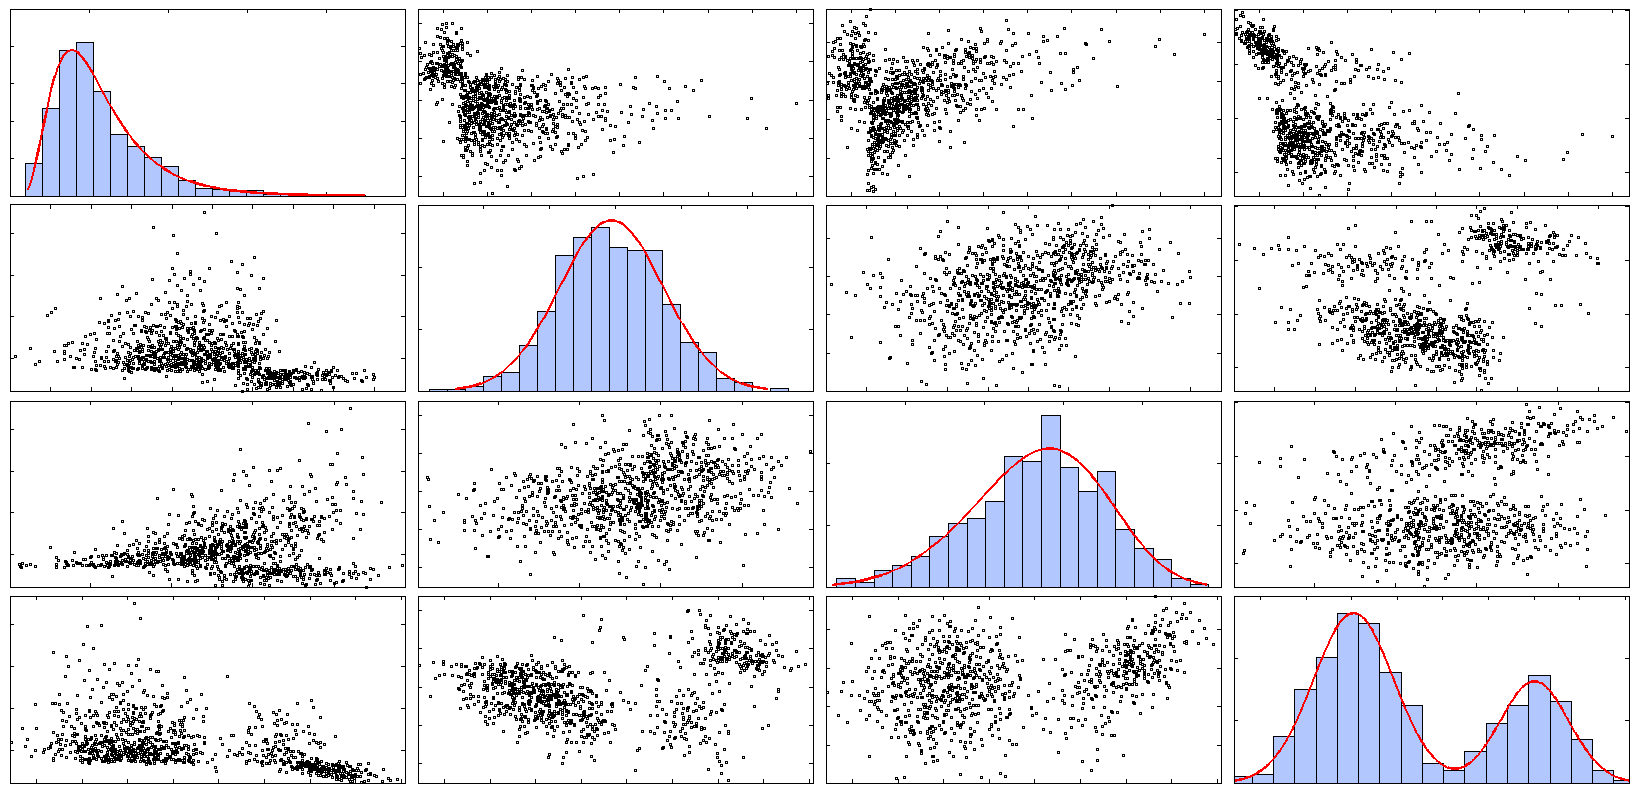
\includegraphics[width= 235pt,height=200pt]{synthetic_data_illustration_new}
\caption{Illustration of the synthetic data used for the analysis. The panels along the diagonal are the marginal histograms with density curves fitted using a parametric family. The best-fit univariate models for the four dimension are log-norm(0,0.05), norm(6,1.5), weibull(2,5) and 0.34*norm(36,2.3)+0.66*norm(28,3.1) respectively. The non-diagonal panel at position $(i,j)$ shows the scatter of data from $i^{th}$ dimension plotted along x-axis and data from $j^{th}$ along the y-axis.}
\label{fig:synthetic_data}
\end{figure}

\begin{figure}[h]
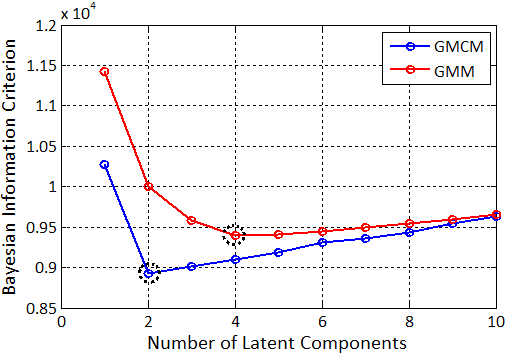
\includegraphics[width= 235pt,keepaspectratio=true]{BIC_GMCM_GMM}
\caption{Model selection procedure for GMMs and GMCMs. The BIC is plotted against the number of mixing components. The best-fit model is the one with lowest BIC as indicated by the dotted circles. GMCMs consistently have lower BIC than GMMs and requires fewer mixing components to model the generative process of the data.}
\label{fig:BIC_comparison}
\end{figure}
For GMMs, we use the standard EM algorithm ~\cite{Bilmes98agentle} and fit models with different number of mixing components ranging from 1 to 10. For each model, we randomly initialize the EM algorithm thirty times and choose a model with lowest BIC. The procedure for fitting GMCM is similar, except that in addition to fitting the Gaussian mixture copula density, we use the parametric marginal distributions shown in figure \ref{fig:synthetic_data}. Figure \ref{fig:BIC_comparison} compares the BIC values of the two models. Clearly, GMCM yields a better fit and requires fewer number of mixing components to achieve that. Note that GMCM have slightly more number of parameters than GMM due to the separate parametric marginal models. 

Figures \ref{fig:gmcm_best_fit} and \ref{fig:gmm_best_fit} show the probability density contours of the best fit GMCM and GMM respectively. The training data is plotted in the background and shown as small black markers.  
\begin{figure}[H]
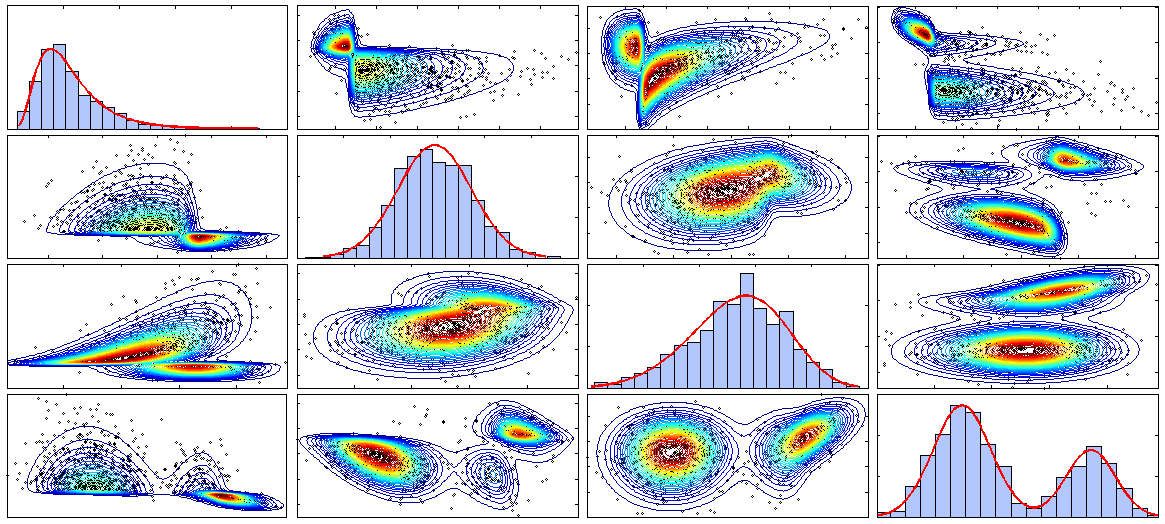
\includegraphics[width= 235pt,height=200pt]{gmcm_best_fit_synthetic_data_contours}
\caption{Contour plots of best-fit GMCM model on the synthetic data. The panels along the diagonals are the marginal histograms with the fitted densities curves. The training data is shown in the background for the visual evaluation of the quality of fit.}
\label{fig:gmcm_best_fit}
\end{figure}
Substantial differences between the two models can be spotted by closely observing the two figures. First, GMCM has a much tighter fit around the data samples and thus appears to be a more faithful generative model of the data. The density of GMM can be seen to diffuse even into those regions with weak or no data support. Secondly, the marginal distributions of fitted GMM may not conform with the true marginal distributions. For instance, the fitted marginal distribution along the first dimension in figure \ref{fig:gmm_best_fit} shows at least two distinct modes, when in fact the true distribution was strictly uni-modal. On the contrary, the GMCM model, by definition, is much more likely to adhere to the true marginal distributions.
\begin{figure}[h]
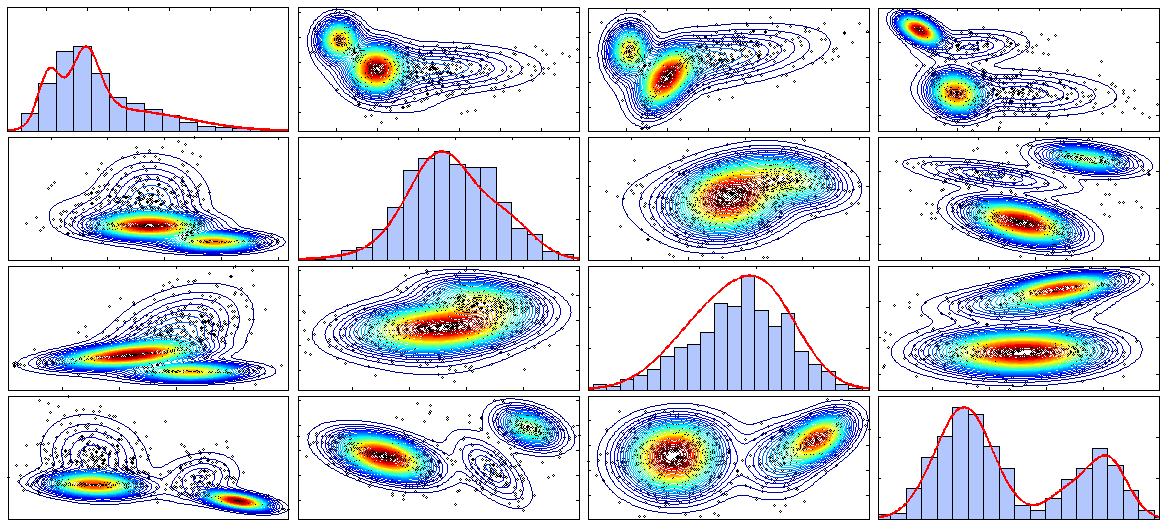
\includegraphics[width= 235pt,height=200pt]{gmm_best_fit_synthetic_data_contours}
\caption{Contour plots of the best-fit GMM model on the synthetic data. The training data is shown in the background for the visual evaluation of the quality of fit. Certain regions, with negligible data-support, have significant probability mass, indicating a relatively inferior fit when compared with GMCM.}
\label{fig:gmm_best_fit}
\end{figure}

In the second experiment, we compare the costs to compute analytical and FD gradients of $Q(\Theta,\hat{\Theta})$. Figure \ref{fig:complexity_comp} plots, on a log-log scale, the CPU time of computing the gradient using the two approaches for different data dimensions.   

\begin{figure}[h]
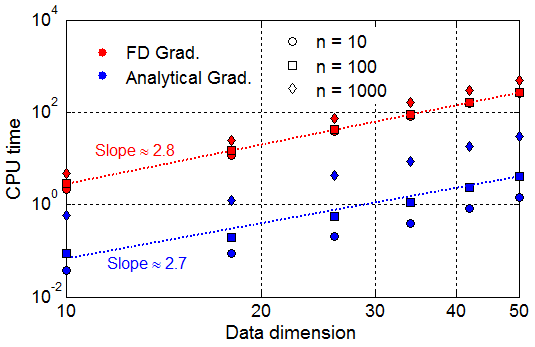
\includegraphics[width= 235pt,height=150pt]{computational_complexity_analytics_vs_fd_grad}
\caption{log-log plots of  the CPU times vs. data dimension for analytical and FD gradient computation of $Q(\Theta,\hat{\Theta})$ function.}
\label{fig:complexity_comp}
\end{figure}
First and foremost, the cubic complexity with $d$ is apparent for both the approaches, from the slopes of the linear fits. We show the linear fits for only the cases where $n=100$. Although both approaches scale similarly with data dimension, we observed at least an order of magnitude of speed-up using the analytical gradients in most cases. The reason being; matrix vector multiplications needed for analytical gradient is an efficient operation with low computational overhead. Secondly, the analytical approach shows higher sensitivity to the number of samples,  $n$, compared to the FD approach. This could be explained based on the asymptotic complexity expressions obtained in Sections \ref{subsec:GMCM_likelihood} and \ref{subsec:complexity_analytic_grad}. For the FD approach the complexity scales as $O\left(m^2d^3g+nmd^3\log{g}\right)$. For small values of $n$, the runtime is dominated by the first term. On the other hand, the complexity of analytical approach is linear in $n$ throughout as it simply adds up the gradient vector over  $n$ data samples. This observation highlights an important practical implication, if a SGD approach is chosen to perform the maximization in the M-step. To be specific, if we obtain analytical gradient using only one data sample and use that to update the parameters, the cost per iteration would scale as $O(md^3)$. However, for FD based gradient the cost remains as $O\left(m^2d^3g\right)$. Depending on the grid size $g$, this difference, could easily add up to a few orders of magnitude of computational cost per iteration. Thus, the ability to compute gradient analytically makes the GMCM parameter learning amenable to SGD approaches to gain further speed up.

In the third and last experiment, we use the SGD approach to learn GMCM parameter on the same data-set used in the first experiment. A notable difference in our implementation  vs. the standard SGD implementation is that we continue to use MATLAB's line-search subroutine to identify the step length. This may be an inefficient strategy and a better heuristics for determining the step length would be more appropriate. However, our goal here to simply provide an evidence that the EM algorithm presented in this paper, when coupled with a SGD approach can significantly speed-up the GMCM learning process.  
\begin{figure}[h]
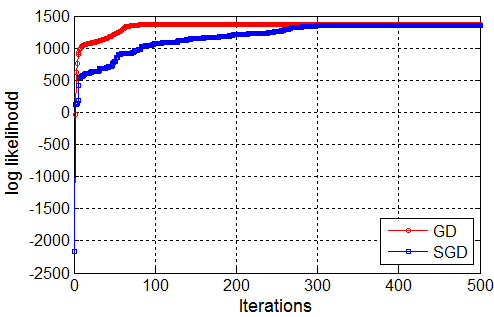
\includegraphics[width= 230pt,height=160pt]{sgd_vs_fgd}
\caption{Illustration of the rate of convergence of the EM algorithm with standard (GD) and the stochastic (SGD) versions of the gradient-descent algorithms. The run-times per iteration were 5.8s and 0.5s for GD and SGD respectively.}
\label{fig:sgd_vs_fgd}
\end{figure}
Figure \ref{fig:sgd_vs_fgd} plots the evolution of log-likelihood function under two scenarios. One where the M-step is carried with the full gradient (GD) information at every iteration of the EM algorithm and one where a single point gradient is used (SGD). The data point for gradient computation is randomly chosen at each iteration. The SGD convergence, albeit slower, catches up with GD and results in a model of similar quality. However, there is a stark difference in the cost per iteration of the two approaches. The GD approach takes 5.8 seconds per iteration, while the SGD approach was an order of magnitude faster, with 0.5 seconds per iteration . 

\section{Conclusion and Future Work}\label{sec:Conclusion&FutureWork}
This paper outlines an EM algorithm for learning the parameters of GMCMs. The GMCM offers a flexible framework and an excellent alternative to GMMs for modeling continuous random variables that exhibit multi-modal distribution with non-Gaussian components. However, learning GMCM parameters is hard owing to its complex likelihood function that does not admit a closed form. As a result, previous algorithms mainly relied on finite-difference (FD) based techniques to maximize the log-likelihood function. The algorithm presented in this paper, obviates the need for numerical gradients whilst improving upon the complexity of previous algorithms. In addition, the ability to compute the gradient of $Q(\Theta,\hat{\Theta})$ function exactly, opens the door to other stochastic versions of the EM algorithm to achieve further speed up and, thus, forms an interesting topic for further research. Another direction of research pertains to expanding the GMCM framework to build better generative models of practical datasets with diverse data types. For instance, GMCMs can be integrated in a mixed graphical modelling framework to model discrete and continuous random variables together. The challenge would be to derive parameter learning and inference algorithms in this setting. A remaining research direction may attempt to modify the present EM algorithm to induce sparsity in the precision matrices of the Gaussian components. This would bring significant benefits in high-dimensional settings where data for training the model is scarce. 

\bibliographystyle{apalike}
\bibliography{Citations_UAI}{}




\end{document}
